\documentclass[aspectratio=169,19pt,english]{beamer}

% =========================================================
\usetheme{Berkeley}
\usecolortheme{default}

\definecolor{PythonBlue}{HTML}{306998}
\definecolor{PythonYellow}{HTML}{FFD43B}
\definecolor{DeepNavy}{HTML}{14213D}
\definecolor{SoftWhite}{HTML}{F7F9FC}
\definecolor{CodeGreen}{HTML}{2A9D8F}

\setbeamercolor{structure}{fg=PythonBlue}
\setbeamercolor{palette primary}{bg=DeepNavy,fg=white}
\setbeamercolor{palette secondary}{bg=PythonBlue,fg=white}
\setbeamercolor{palette tertiary}{bg=DeepNavy,fg=white}
\setbeamercolor{palette quaternary}{bg=PythonBlue,fg=white}
\setbeamercolor{title}{fg=white,bg=DeepNavy}
\setbeamercolor{frametitle}{fg=white,bg=DeepNavy}
\setbeamercolor{block title}{fg=white,bg=PythonBlue}
\setbeamercolor{block body}{fg=DeepNavy,bg=SoftWhite}
\setbeamercolor{alerted text}{fg=PythonBlue}
\setbeamercolor{normal text}{fg=DeepNavy,bg=white}
\setbeamercolor{item}{fg=PythonBlue}
\setbeamercolor{section in toc}{fg=PythonBlue}
\setbeamercolor{bloqueder}{bg=red!20, fg=black}
\setbeamercolor{bloquetitder}{bg=red, fg=white}

\setbeamercolor{bloqueizq}{bg=blue!20, fg=black}
\setbeamercolor{bloquetitizq}{bg=blue, fg=white}
\setbeamertemplate{navigation symbols}{}
\setbeamertemplate{items}[triangle]
\setbeamertemplate{blocks}[rounded][shadow=false]


\setbeamercovered{invisible}

% =========================================================
% PACKAGES
% =========================================================
\usepackage[T1]{fontenc}
\usepackage[utf8]{inputenc}
\usepackage{babel}
\usepackage{lmodern}
\usepackage{microtype}
\usepackage{enumitem}
\usepackage{graphicx}
\usepackage{booktabs}
\usepackage{mathtools}
\usepackage{amssymb}
\usepackage{xcolor}
\usepackage{listings}
\usepackage{tikz}
\usepackage{hyperref}
\usepackage{listings}
% =========================================================
% PYTHON CODE STYLE
% =========================================================
\lstdefinestyle{pythonstyle}{
	language=Python,
	basicstyle=\ttfamily\small,
	keywordstyle=\color{PythonBlue}\bfseries,
	stringstyle=\color{CodeGreen},
	commentstyle=\color{gray}\itshape,
	numbers=left,
	numberstyle=\tiny\color{gray},
	numbersep=8pt,
	showstringspaces=false,
	breaklines=true,
	frame=single,
	rulecolor=\color{PythonBlue!25},
	backgroundcolor=\color{SoftWhite},
	tabsize=4,
	keepspaces=true,
	columns=fullflexible
}
\lstset{style=pythonstyle}

% =========================================================
% metadata
% =========================================================
\title[CLASS 3.]{Introduction to Programming}
\subtitle{Python Fundamentals}
\author[ ]{Luis Ángel Bustos Ochoa}
\institute{Applied Physics}
\date{\today}

% =========================================================
% DOCUMENT
% =========================================================
\begin{document}
	
	% ---------------------------------------------------------
	% FRAME 1 — TITLE PAGE  ---------------------------------------------------------
	{
		\setbeamercolor{background canvas}{bg=DeepNavy}
		\begin{frame}[plain]
			\centering
			\vspace{0.7cm}
			
			{\color{PythonYellow}\rule{0.22\textwidth}{2pt}}
			
			\vspace{0.65cm}
			
			{\color{white}\Huge\bfseries Introduction To Programming\par}
			
			\vspace{0.35cm}
			
			{\color{PythonYellow}\Large Python fundamentals\par}
			
			\vspace{0.8cm}
			
			\begin{tikzpicture}
				\node[
				rounded corners=8pt,
				fill=white,
				text=PythonBlue,
				inner sep=14pt
				] {
					\begin{minipage}{0.58\textwidth}
						\centering
						\ttfamily\Large
						Universidad...
					\end{minipage}
				};
			\end{tikzpicture}
			
			\vfill
			
			{\color{white}\large Luis Ángel Bustos Ochoa\par}
			\vspace{0.15cm}
			{\color{white!75}\normalsize Class 3 \textbar{} Course: \par}
			
			\vspace{0.55cm}
			{\color{PythonYellow}\rule{0.22\textwidth}{2pt}}
			
			\vspace{0.35cm}
			{\color{white!70}\small\insertdate\par}
		\end{frame}
	}	
	%
	\section{Introduction}
	{\Large
		\begin{frame}{Today's Goals}
			
			\begin{itemize}
				\item[---]More about strings
				%\item Algorithms 
				\item[---] Advance strings operations 
				\item[---] Input and interaction with the user
				
			\end{itemize}
		\end{frame}
		
		\begin{frame}{Are each of the following valid string objects in python?}
			\begin{enumerate}[label=\Roman*.]
				\item "888"
				\item "a string"
				\item "a very very long string with a lot of symbols@sfaj4-sjo\_!"
				\item 'combo'
				\item hello
				\item ""
			\end{enumerate}
		\end{frame}
		
		\begin{frame}{"Structure of a string"}
			\framesubtitle{Indexation.}
			The most basic operation you can do with a string is called 'indexing', this determinate the value of a character at a certain position in the string.
			
			
		\end{frame}
		\begin{frame}
		 
		 \begin{figure}{Example}
		 	\centering
		 	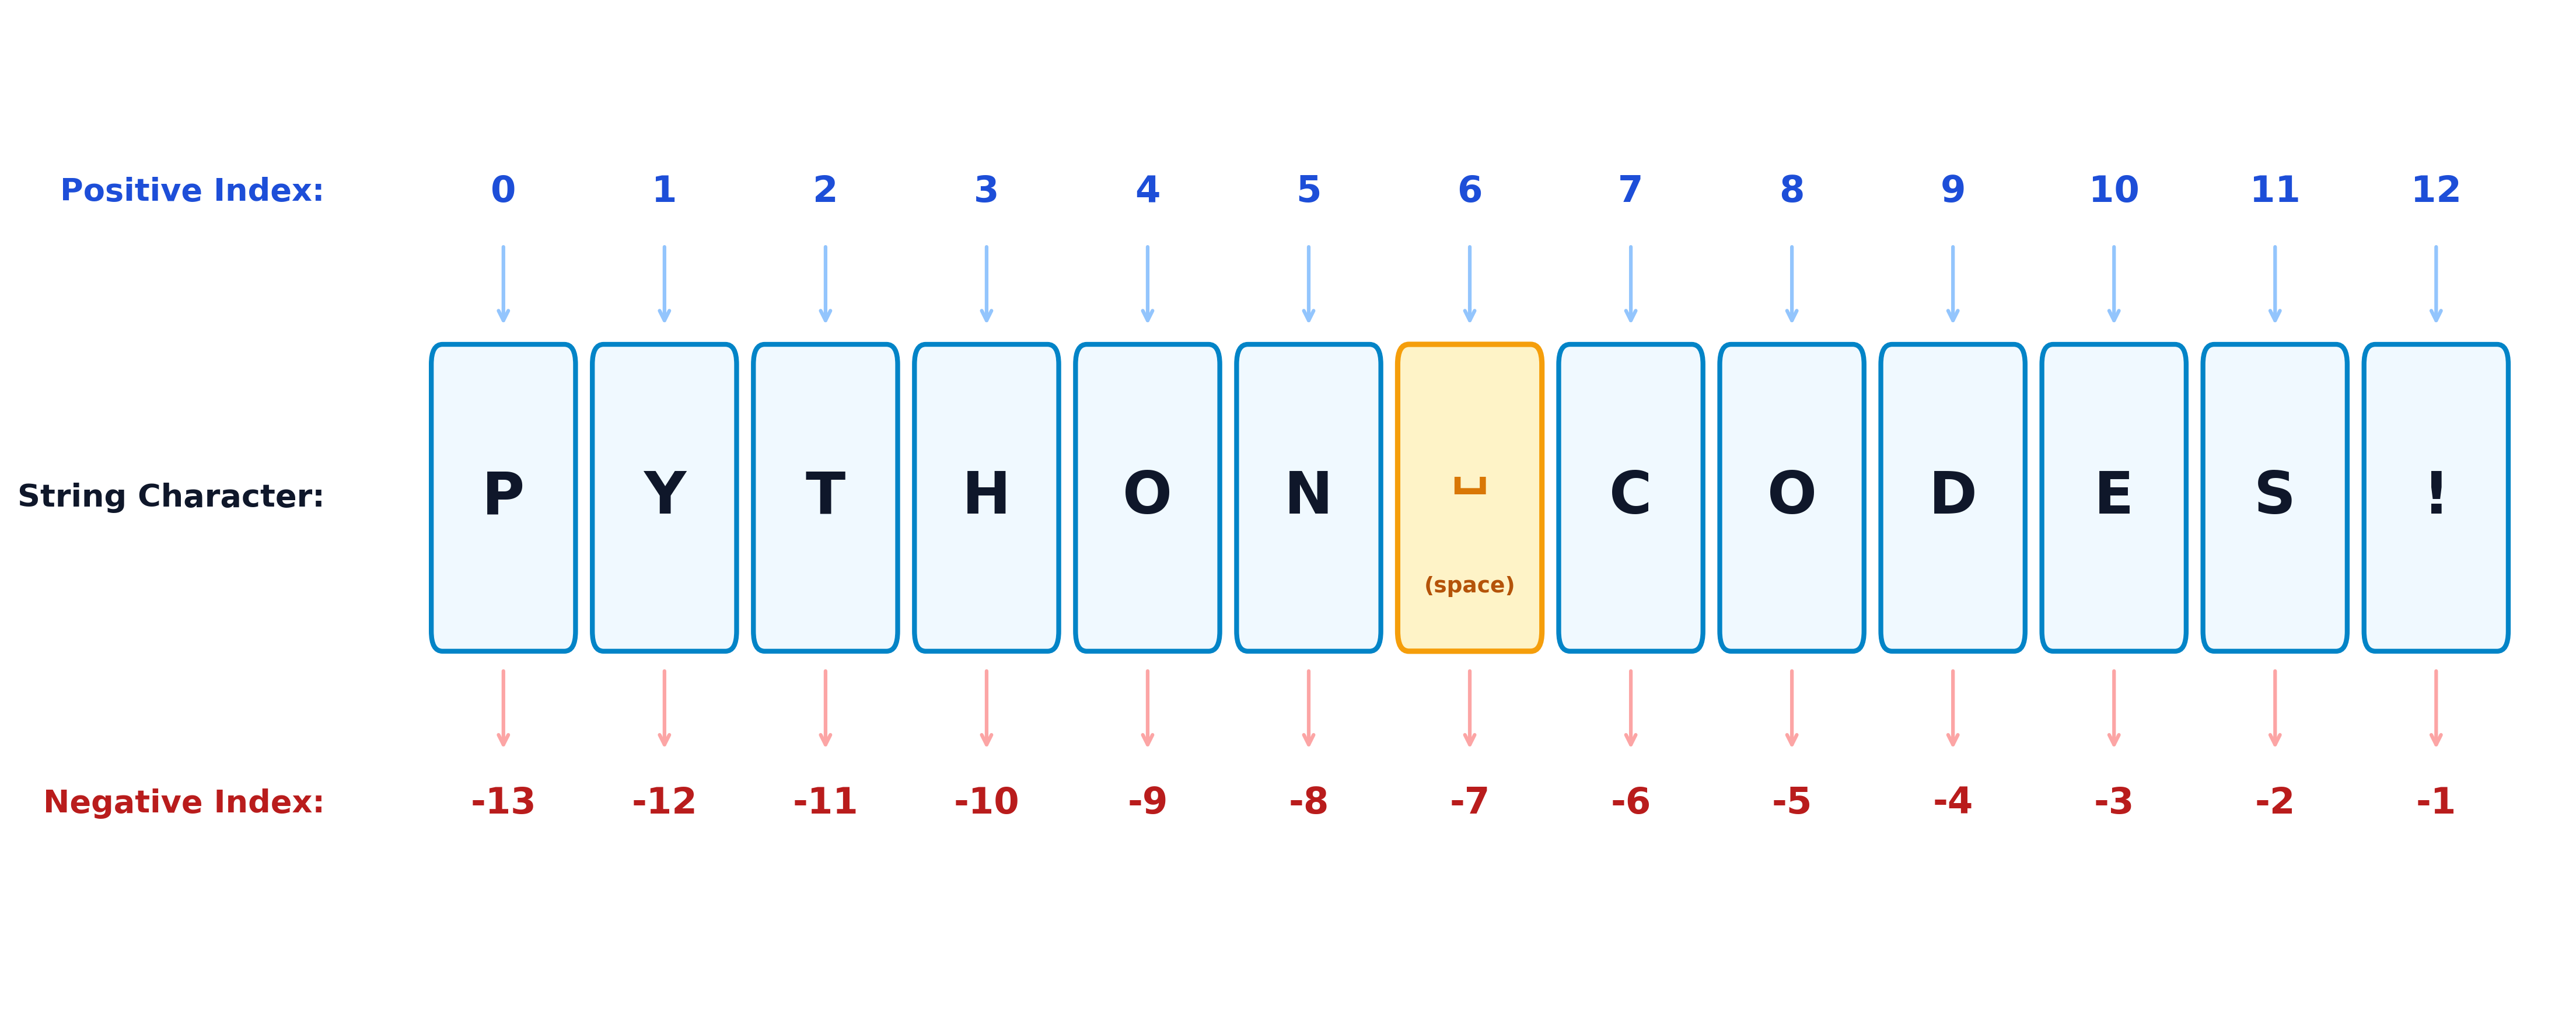
\includegraphics[width=9cm]{string_indexing_boxes_v2.png}
		 	\label{fig:stringindexingboxesv2}
		 \end{figure}
		 \textit{
		 -Start at 0. \\
		 - The last character "!" is at index 12. \\
		 -You can also count backward. The last character in any string is always at index -1 when you are counting backward. 
		}
		\end{frame}
%		\begin{frame}{If you shouldn't be familiar with the Flowcharts}
%			\framesubtitle{You should be familiar with following a set of instructions and making branching desicions.}
%			\begin{figure}
%				\centering
%				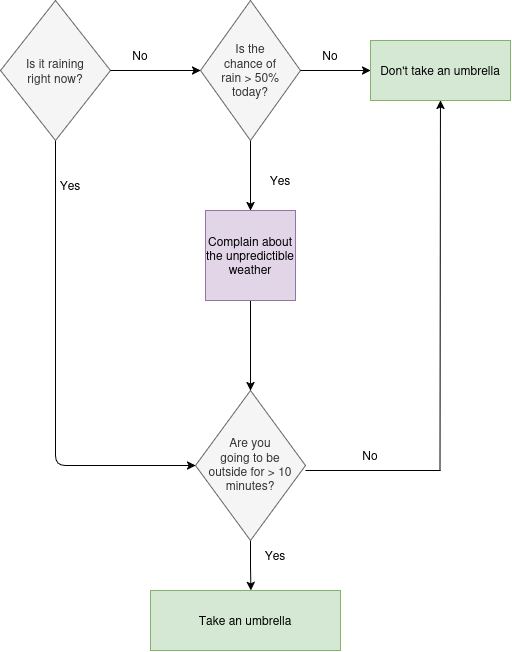
\includegraphics[width=6.9cm, height=6.55cm]{diagram.png}
%				
%			\end{figure}
%			
%		\end{frame}
		\begin{frame}
			
		For the string '4 ever'. What is the index number of the following characters? Give the forward and backward index value.
		\begin{enumerate}[label=\roman*.]
			\item 4
			\item v
			\item r
		\end{enumerate}
		\end{frame}
		
		\begin{frame}{Slicing a string}
			\framesubtitle{If you want to known the value of a group characters...}
		 You can get a substring of the string. To slice a string, you can put up to three integers, separated by colons, in squared brackets.
		 \begin{center}
		 	\Large{\textbf{[Start index: stop index: step]}}
		 	\textit{you can use "negative steps" and if you omitted, the step is equal to 1}
		 \end{center}
		 
		\end{frame}
		
		\begin{frame}{Example}
			\framesubtitle{s=PYTHON CODES!}
			\begin{center}
				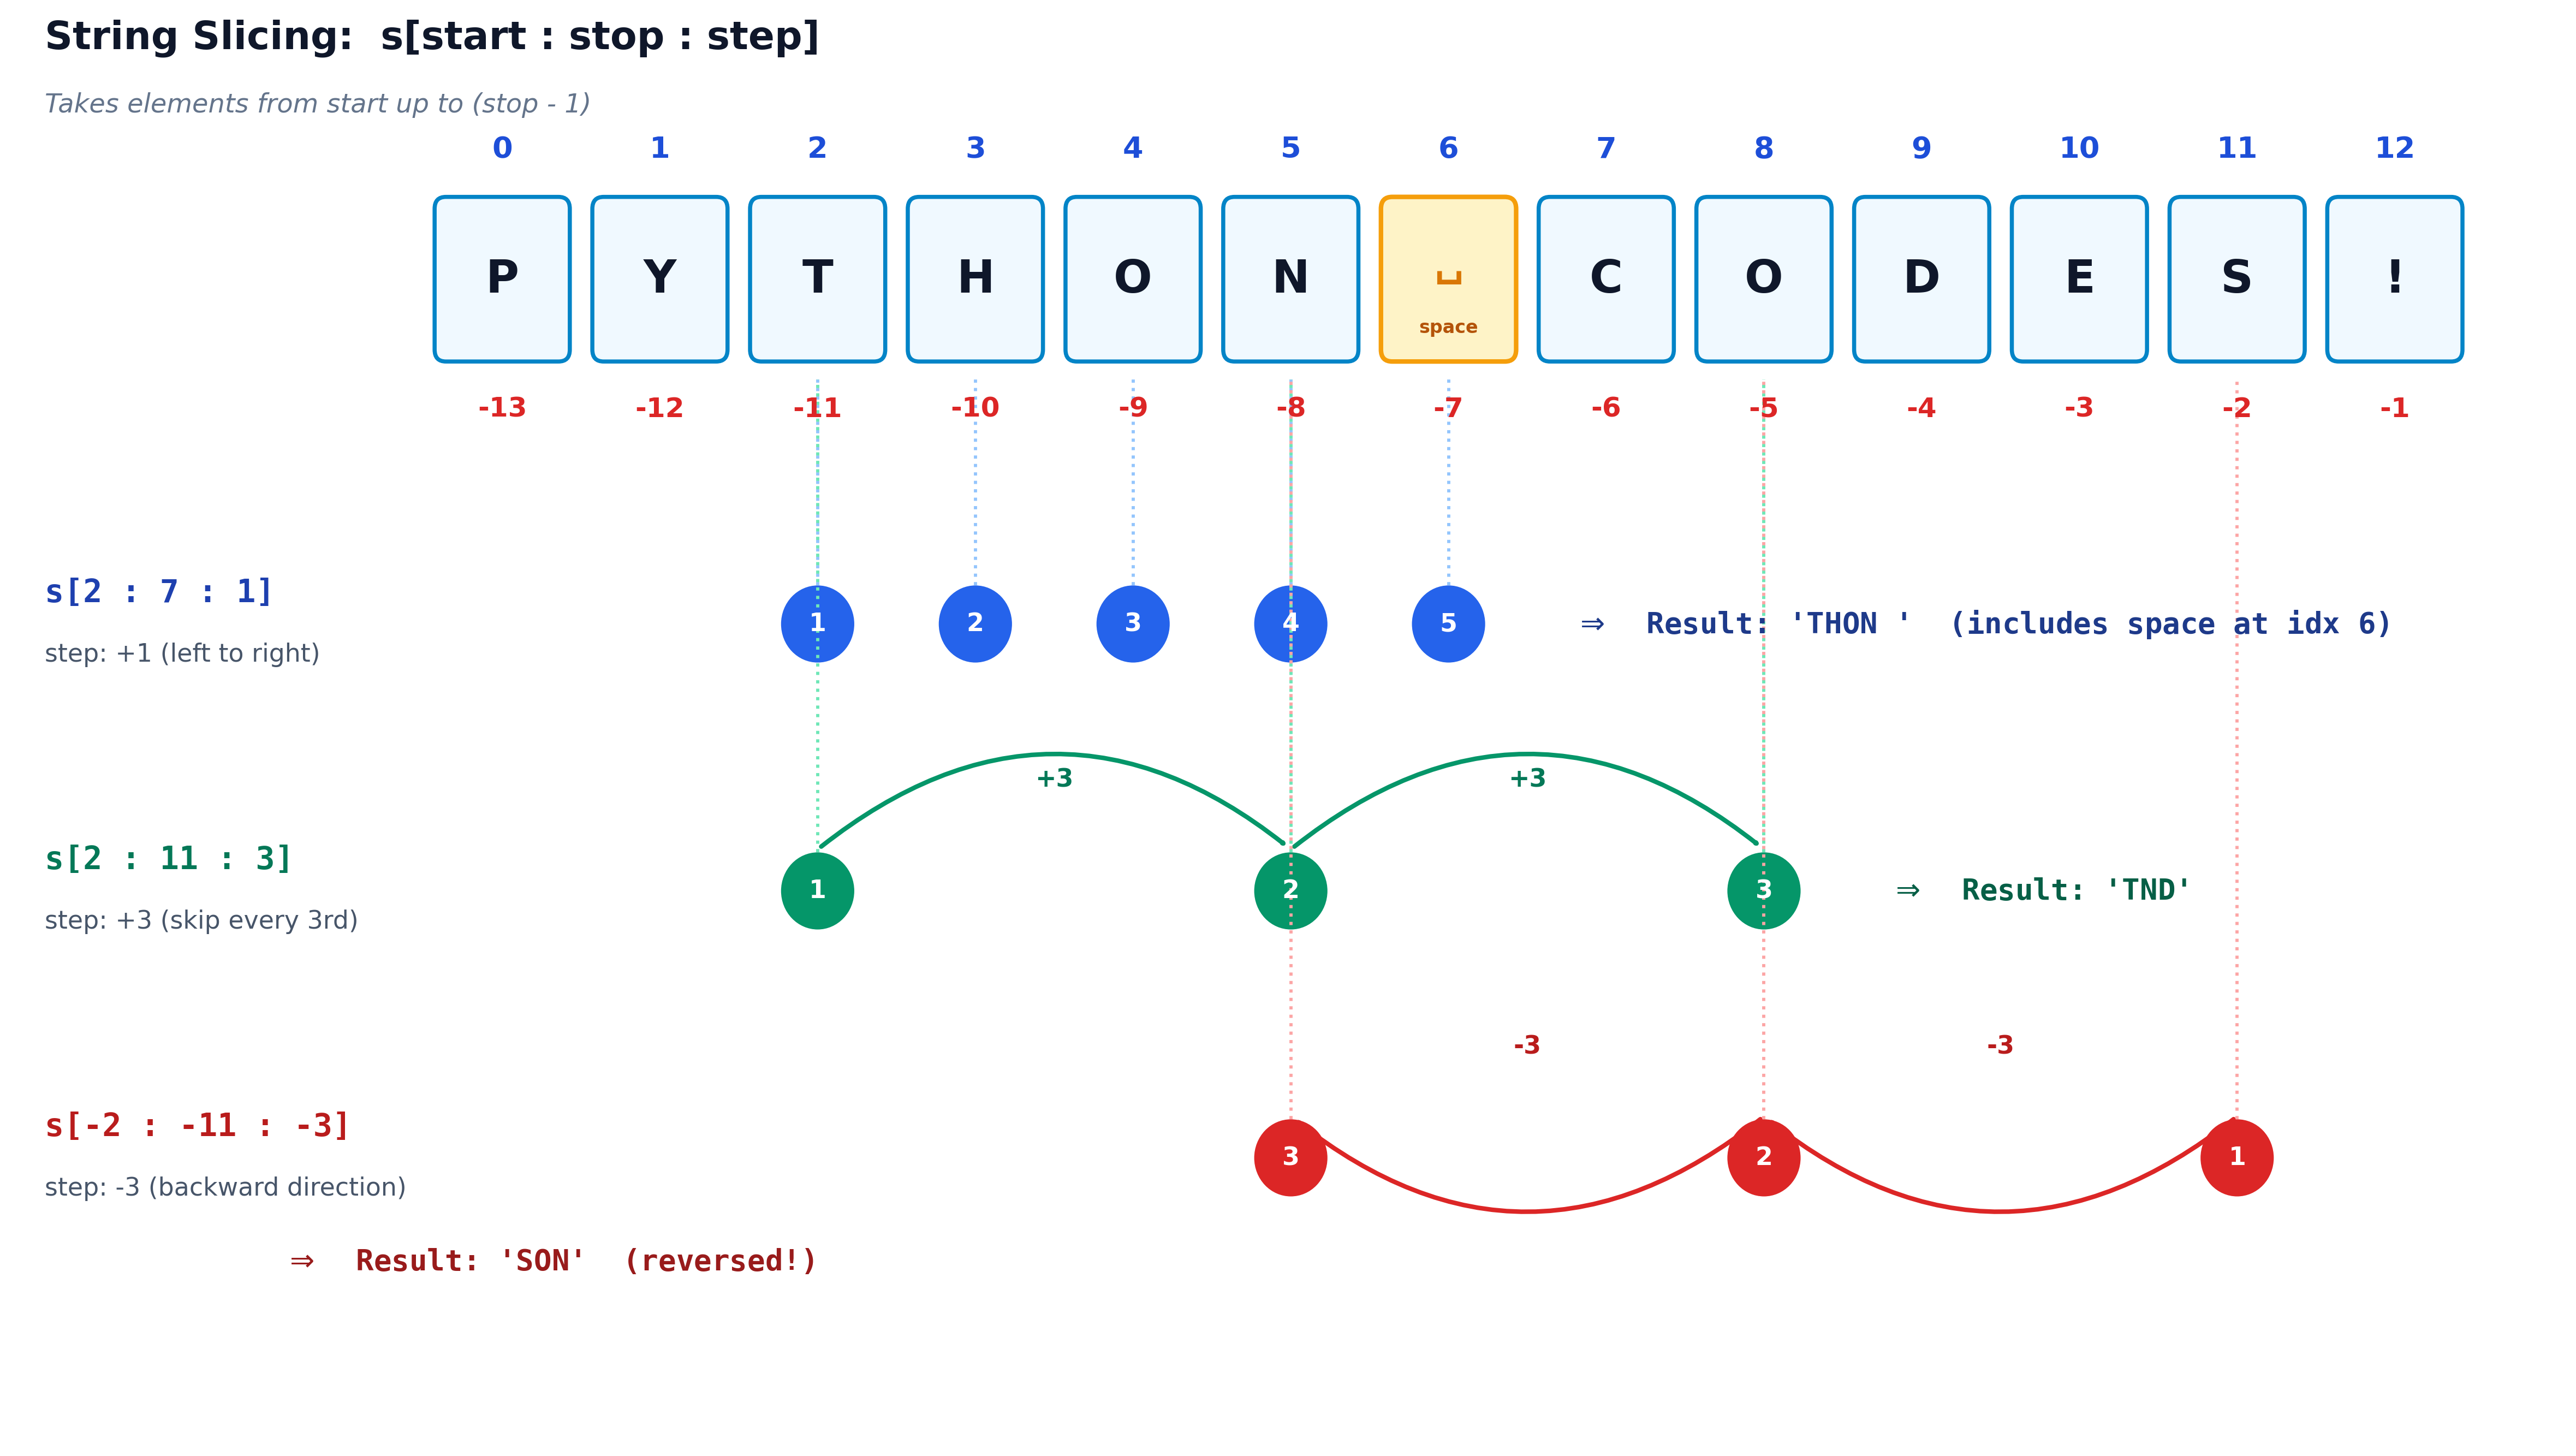
\includegraphics[width=11cm]{string_slicing_diagram}
			\end{center}
			
		\end{frame}
		\section{Operations}
		\begin{frame}{len()}
			you can use len(), to get the number of characters in the string (the command len() can be apply to another type of objects).
			\begin{itemize}[label=$\diamond$]
				\item len ("") evaluates to 0.
				\item ("Boston 4 ever") evaluates to 13.
				\item a="hi!", then len(a) evaluates to 3.
			\end{itemize} 
			
		\end{frame}
		\begin{frame}{upper(),lower (), title() and capitalize() ...}
		\framesubtitle{And introduction to the dot notation.}
			The next operations that you can do on strings will take on a different look. 
			The dot notation only works on a specific type of object. This touches upon a much deeper idea called: "object-oriented programming"; we will se it in another lesson. \\
			
		\end{frame}
		\begin{frame}{upper(),lower () and title(), Capitalize()}
			These commands affect only the letter characters in the string, numbers and other characters in the string are not affected. 
			\begin{enumerate}[label=\arabic*.-]
				\item 'A'\textit{\textbf{.lower()}} evaluates to 'a'
				\item 'a'\textit{\textbf{.upper()}} evaluates to 'A'
				\item 'Ups\_and Down'\textbf{\textit{.swapcase()}} evaluates to 'uPS\_ AND dOWN '
				\item 'a long time...'\textbf{\textit{.capitalize()}} evaluates to 'A long time...'
				\item "a long time...."\textbf{\textit{.Title()}} evaluates to 'A long Time...'
			\end{enumerate}
		\end{frame}
		\begin{frame}{More operations...}
			\begin{itemize}
				\item[*] strip()
				\item[*] rstrip()
				\item[*] lstrip()
				\item[*] find()
				\item[*] in
				\item[*] replace
				\item[*] count
			\end{itemize}
		\end{frame}
		\section{Formats}
		\begin{frame}{f'using variable strings'}
		\framesubtitle{To insert variable's value into a string, we used the f an then quotation mark}
		\begin{center}
			
		
		first\_name= "yin"\\
		last\_name="yan"\\
		full=f'{first\_name} {last\_name}'\\
		message=f"Hello,{full.title()}!"\\
		print(message) 
	\end{center}
		note: try to use f" " instead of f' ' and the same with any string.

		\end{frame}
		\section{Input()}
		\begin{frame}{input()}
			\framesubtitle{Interacting with the user with input()}
			In Python, input("write the thing that you need here!") only returns string data.
		\end{frame}
		\begin{frame}{Exercises}
			\begin{enumerate}[label=\arabic*.-]
				\item Write  program that asks the user's name and then age, them calculate how old the user will be in 30 years. 
				\item Write one or more commands that uses the string "Greater" to get "ATE".
				\item Write a program that initializes a variable string with the value "Eating,work\_play Repeat". Then, get the string "working playing" manipulating the variable 
			\end{enumerate}
			
		\end{frame}
	}
\end{document}